\section {Experimental setup}
We propose to carry out the new measurement using the Soenoidal Large Intensity Device (SoLID~\cite{solid_pcdr}), in parallel with the already approved experiment, E12-10-006~\cite{solid:e12-10-006}, which will measure the Semi-Inclusive Deep-Inelastic Scattering (SIDIS). There are two SoLID configurations, called the SoLID-SIDIS and SoLID-PVDIS. Besides E12-10-006, two SIDIS experiments, E12-11-007~\cite{solid:e12-11-007} and E12-11-108~\cite{solid:e12-11-108}, along with the $J/\psi$ experiment (E12-12-006~\cite{solid:e12-12-006}), will use the SoLID-SIDIS configuration. All these experiments have been approved with A or A- rating. In addition, two "bonus-run" experiments, E12-10-006A~\cite{solid:e12-10-006A} and E12-11-108A~\cite{solid:e12-11-108A}, have also been approved to run in parallel with the SIDIS experiments. The SoLID-PVDIS configuration is for the Parity Violation in Deep Inelastic Scattering (PVDIS).

The experiment will use a near identical setup as E12-10-006, but with few additions without affecting the approved experiment. We will use exactly the same online production trigger, which is the coincidence of electron triggers and hadron triggers. However, we request to add a new trigger type on top of the existing ones to identify the proton events for the offline triple coincidence analysis. The SoLID-SIDIS detector can only detect protons with scattering angles from 8$^{\circ}$ up to 24$^{\circ}$, while the main proton events from the DVMP process can cover up to 65$^{\circ}$. We propose to add a new proton detector based on scintillator counters  to detect protons from  24$^{\circ}$ to  65$^{\circ}$. The new detector will be placed between the target system and the entrance and of CLEO-II magnet. The new proton trigger and the new proton detector will be discussed in more detailed in the following sections.

\subsection {Transversely Polarized $\mathrm{^{3}He}$ Target}
\begin{table}[!ht]
\centering
\begin{tabular}{|c|c|}
\hline
Target                       & $^3$He              \\\hline 
Length                       & 40 cm               \\\hline          
Target Polarization          & $\sim$60\%          \\\hline 
Target Spin Flip             & $\leq$20 mins       \\\hline 
Target Dilution              & 90\%  \\\hline
Effective Neutron            & 86.5\%  \\\hline
Target Polarimetry Accuracy  & $\sim$ 3\%          \\\hline
\end{tabular}
\caption{\footnotesize{Key Parameters of the $\mathrm{^{3}He}$ target.}}\label{table:target}
\end{table} 
The proposed measurement will utilize the same polarized $\mathrm{^{3}He}$ as E12-10-006~\cite{e12-10-006}. Such a target was successfully employed in E06-110, a 6~GeV SIDIS experiment in Hall A. The polarization direction is held by three sets of Helmholtz coils with a 25~Gauss magnetic filed. Both the transverse and longitudinal directions can be provided by rotating the magnetic field. The $\mathrm{^{3}He}$ gas with density of about 10~atm (at $0^{\circ}$) is stored in a 40~cm target cell made of thin glasses. With a 15~$\mu A$ electron beam, the neutron luminosity can be as high as $10^{36} cm^{-2}s^{-1}$. The in-beam polarization of 60\% was archived during the E06-110 experiment. Two kinds of polarimetry, NMR and EPR, were used to measure the polarization with relative 5\% precision. We have planed to improve the accuracy of the measurement to reach 3\%.

The target spin will be reversed for every 20 minutes by using the RF AFP technique. The additional polarization loss due to the spin reversal was kept at $<10~\%$ which has been taken into account in the overall 60\% in-beam polarization. A new method for spin reversal using filed rotation has been tested and was able to eliminate the polarization loss. Such an improvement will enable us to perform the spin-reversal in few minutes to reduce the target-spin-correlated systematic errors. The key parameters of the $\mathrm{^{3}He}$ target are summarized in Table~\ref{table:target}.
  
A collimator, similar to the one used in the E06-110, will be placed next to the target cell window to minimize the target cell contamination and to reduce the event rate. Several calibration targets will also be installed in this target system, including a multi-foil $^{12}C$ for optics study, a BeO target for beam tuning, and a reference target cell for dilution study and other calibration purposes.
  
\subsection {SoLID Spectrometer and Detectors} 
The solenoid magnet for SoLID will be based on the CLEO-II magnet built by Cornell University. The magnet is 3 meters long with the out diameter of 3 meters and the inner diameter of 1 meter. The field strength is greater than 1.35 Tesla with integrated BDL of 5 Tesla-meters. The fringe filed at the front end after shielding is less than 5 Gauss. In the SIDIS-configuration, the CLEO-II magnet provides 2$\pi$ acceptance in the azimuthal angle ($\phi$) and covers the polar angle ($\theta$) from 8$^{\circ}$ up to 24$^{\circ}$. The momentum acceptance is between 0.8 and 7.5~GeV/c and the resolution is about 2\%. 

\begin{figure}[!ht]
 \begin{center}
  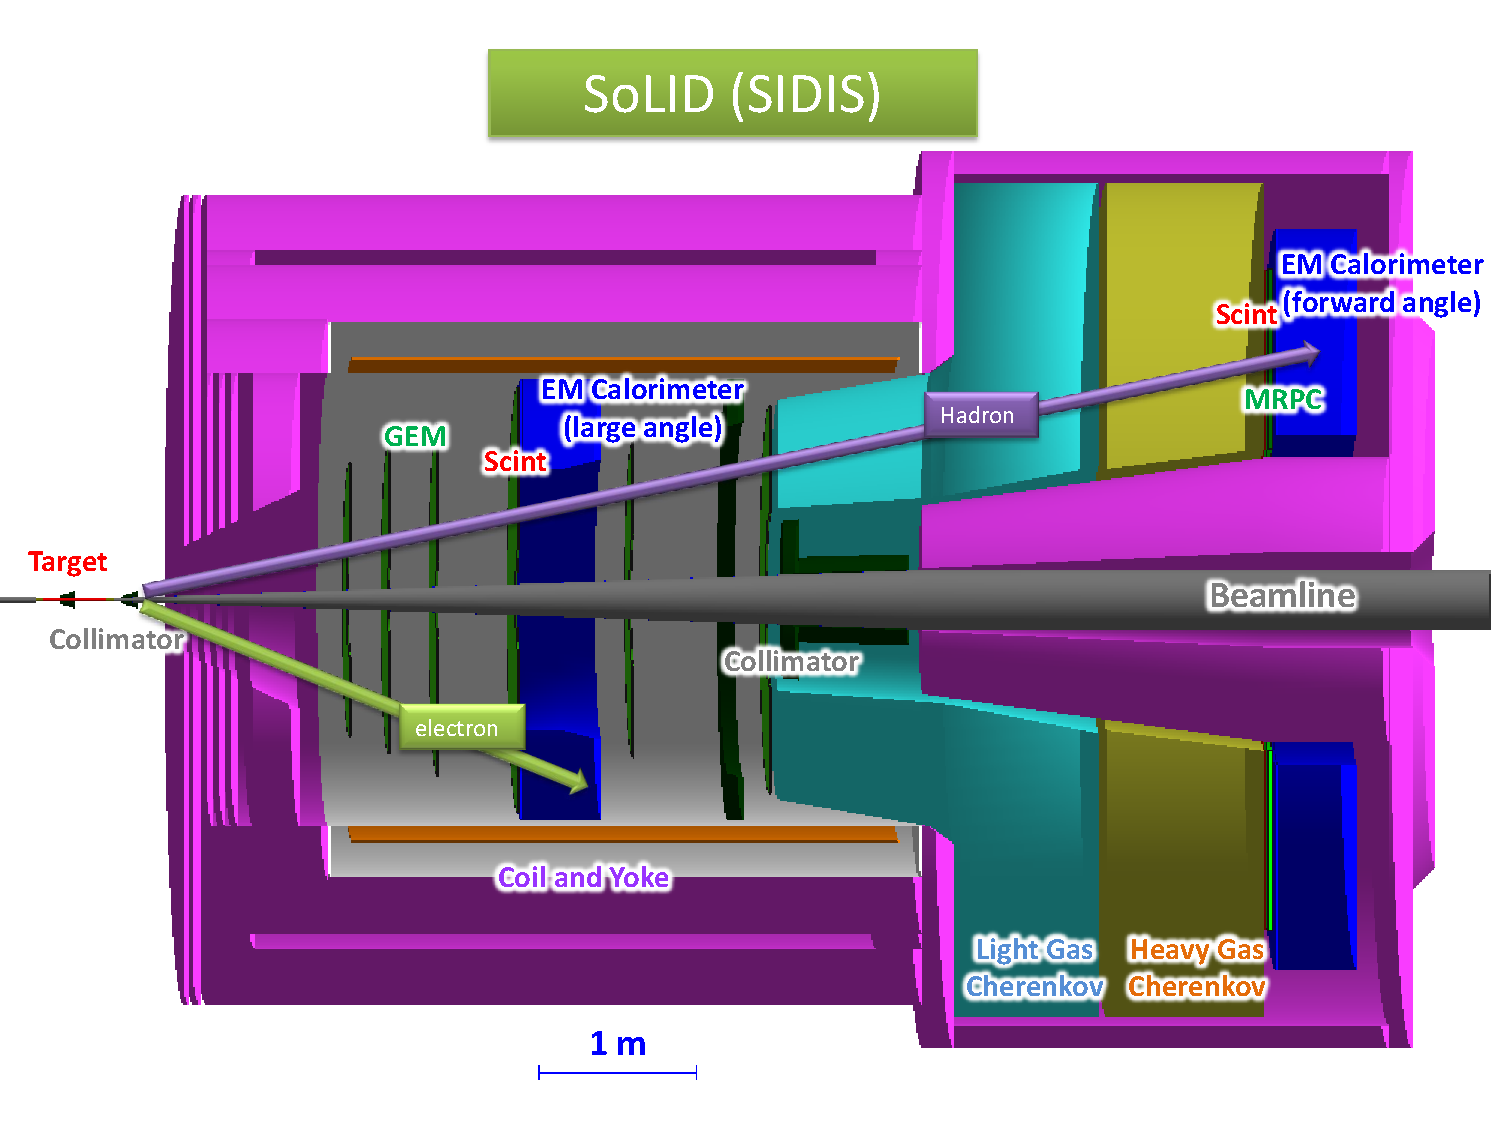
\includegraphics[width=0.8\textwidth]{./figures/SoLID_SIDIS_setup.pdf}
   \caption[The Detector Layout of the SoLID-SIDIS configuration]{\footnotesize{The Detector Layout of the SoLID-SIDIS configuration. The detector system includes six Gas Electron Multiplier (GEM) planes for charged particle tracking, two Scintillator Pad Detectors (SPD) followed by two Shashlyk sampling EM Calorimeters (EC) for energy measurement and particle identification, a Light Gas \v{C}erenkov Detector (LGC) for e-$\pi^{\pm}$ separation, a Heavy Gas \v{C}erenkov Detector (HGC) for $\pi^{\pm}$-$K^{\pm}$ separation, as well as a Multi-gap Resistive Plate Chamber (MRPC) for timing measurement. The first four GEM trackers, the first SPD (i.e. LASPD) and EC (i.e. LAEC) form the large-angle detection system for electron measurement. The forward-angle detection system, to measure electron and hadrons, is composed of all six GEM trackers, LGC, HGC, MRPC, the second SPD (i.e. FASPD) and the second EC (FAEC). The photon-detection in the large-angle is given by the veto-signal of the SPD in coincidence with the EC signal, where the photons in the forward-angle system will be triggered by the EC signal plus the veto-signals of LGC, SPD, and MRPC.}}
   \label{solid_sidis}
 \end{center}
\end{figure}

The layout of the SoLID detectors in the SIDIS-configuration is shown in Fig.~\ref{solid_sidis}. The detector system is divided into two regions for the forward-angle (FA) detection and the large-angle (LA) detection. Six Gas Electron Multiplier (GEM) tracking chambers will be used for charged particle tracking, where only the first four of them will be used for the large-angle detection. In each region, a Shashlyk-type sampling EM calorimeter (LAEC or FAEC) will measure the particle energy and identify electrons from hadrons. A scintillator-pad detector (LASPD and FASPD) will be installed in front of each EC to reject photons and provide timing information. The forward-angle detectors will detect both the electrons and hadrons (mainly $\pi^{\pm}$). A light-gas \v{C}erenkov detector (LGC) and a heavy-gas \v{C}erenkov detector (HGC) will perform the $e/\pi^{\pm}$ and $\pi^{\pm}/K^{\pm}$ separation, respectively. The Multi-gas Resistive Plate Chamber (MRPC) will provide a precise timing measurement and serve as a backup of the FASPD on photon rejection. A more detailed discussion of the design, simulation, prototype-test of each detector is given in the SoLID preliminary conceptual design report (pCDR)~\cite{solid_pcdr}. 

Table~\ref{table:key_par_sidis_dvcs} summarizes the key parameters of the detector system in the SIDIS configuration for both the SIDIS and DVMP measurements. 
\begin{table}\centering
\begin{tabular}{|c|c|c|c|c|}
\hline
Experiments                             & SIDIS                 & DVMP  \\\hline
Reaction channel                     &  $\vec{n}(e,e'\pi^{\pm})X$    & $\vec{n}(e,e'\pi^{-})p$	\\\hline
Target                                       & $^3$He                &same 	\\\hline
Unpolarized luminosity             & $\sim10^{37}$ cm$^{-2}$s$^{-1}$        & same	\\\hline 
Momentum coverage (GeV/c)  & 0.8-7.5               &same 	\\\hline
Momentum resolution              &  $\sim$2\%            & same\\\hline
Azimuthal angle resolution      & 5 mr                  & same	\\\hline
Polar angle coverage              &  8$^{\circ}$-24$^{\circ}$ for $e$                 &  same \\\hline
Polar angle coverage              &  8$^{\circ}$-14.8$^{\circ}$ for $\pi^{\pm}$  &  same 	\\\hline
				                                 &                                                        & 8$^{\circ}$-24 $^{\circ}$ for $p$         \\\hline
   				                                 &                                                        & 24$^{\circ}$-65 $^{\circ}$ for $p$ with recoil detector         \\\hline
 Polar angle resolution             & 0.6 mr                & same	\\\hline
Target Vertex resolution          & 0.5~cm                & same \\\hline
 Energy resolution on ECs      & 5\%$\sim$10\%         & same   \\\hline
Trigger type                             & Double Coincidence $e^-+\pi^{\pm}$ & Tripple Coincidence $e^-+\pi^{-}+p$\\\hline
Expected DAQ rates               &  $<$100 kHz           &  same online ($<$30 Hz offline)\\\hline
Main Backgrounds                  & (e,e'K$^\pm$)        &(e,e'$\pi^{\pm}$) \\
                                                &   Accidental Coincidence      & Accidental Coincidence	\\\hline
Key requirements                      &  Radiation hardness   & Radiation hardness	\\
                                             &  Kaon Rejection   & Proton Detection	\\
                                              &  DAQ                  &       \\
                        \hline
\end{tabular}
\caption{\footnotesize{Summary of Key Parameters for DVCS Measurement compared with SIDIS Experiments.}}\label{table:program_summary}
\label{table:key_par_sidis_dvcs}
\end{table} 

\subsection{A Proton Recoil Detector}
In the SoLID-SIDIS detector system, protons can be isolated from rest of hadron events by using the time-of-fly (TOF) information which requires the timing to be as good as {\bf 100} ps ({\bf Check it!}). 



\subsection{Trigger Design}
In E12-10-006, the online production trigger will be the double-coincidence of the scattered electrons and hadrons. One will use the particle identification detectors, such as LGC, HGC and ECs, during the offline analysis to select $\pi^{\pm}$ out from hadrons. The DVMP events will be identified with the triple-coincidence trigger of the scattered electron, $\pi^{-}$ and proton. We will use the same online trigger as the SIDIS one, and hence the new experiment will share the same data set as E12-10-006. However, a new trigger type will be added to the DAQ system to record protons events, and we will perform the offline analysis to isolate the triple-coincidence events.. 

The proton trigger will be produced in two regions, the new proton recoil detector and the standard SoLID timing detectors (e.g., MRCP and LASPD). 

The actual trigger design will be far more complicated, and the detailed discussion of the trigger and DAQ design has been given in the SoLID pCDR~\cite{solid_pcdr}.
